
%% bare_conf.tex
%% V1.3
%% 2007/01/11
%% by Michael Shell
%% See:
%% http://www.michaelshell.org/
%% for current contact information.
%%
%% This is a skeleton file demonstrating the use of IEEEtran.cls
%% (requires IEEEtran.cls version 1.7 or later) with an IEEE conference paper.
%%
%% Support sites:
%% http://www.michaelshell.org/tex/ieeetran/
%% http://www.ctan.org/tex-archive/macros/latex/contrib/IEEEtran/
%% and
%% http://www.ieee.org/

%%*************************************************************************
%% Legal Notice:
%% This code is offered as-is without any warranty either expressed or
%% implied; without even the implied warranty of MERCHANTABILITY or
%% FITNESS FOR A PARTICULAR PURPOSE! 
%% User assumes all risk.
%% In no event shall IEEE or any contributor to this code be liable for
%% any damages or losses, including, but not limited to, incidental,
%% consequential, or any other damages, resulting from the use or misuse
%% of any information contained here.
%%
%% All comments are the opinions of their respective authors and are not
%% necessarily endorsed by the IEEE.

\documentclass[a4paper]{article}


\usepackage{natbib}
\usepackage{amsmath}
\usepackage{subfigure}
\usepackage{graphicx}
\usepackage{graphics}
\usepackage{pstricks,pstricks-add}
\newcommand{\figurepath}{Figures}

\newcommand{\titlesize}{\fontsize{16pt} \selectfont}


\begin{document}
%
% paper title
% can use linebreaks \\ within to get better formatting as desired
\title{\titlesize \bf Adaptive Character Motion Synthesis By Qualitative Approach}

\author{
Fangde Liu\\
\\National Center For Computer Animation\\Media School\\
\\Bournemouth University\\
Email: fliu@bmth.ac.uk
\and
Xiaosong Yang\\
NCCA\\Media School\\
Bournemouth University\\
xyang@bournemouth.ac.uk
\and
Jianjun Zhang 
NCCA\\Media School\\
Bournemouth University\\
jzhang@bournemouth.ac.uk
}


% author names and affiliations
% use a multiple column layout for up to three different
% affiliations
%\author{\IEEEauthorblockN{Fangde Liu}
%\IEEEauthorblockA{National Center For Computer Animation\\Media School\\
%Bournemouth University\\
%Email: fliu@bmth.ac.uk}


%\and

%\IEEEauthorblockN{Xiaosong Yang}
%\IEEEauthorblockA{NCCA\\Media School\\
%Bournemouth University\\
%xyang@bournemouth.ac.uk
%}
%\and
%\IEEEauthorblockN{Jianjun Zhang}
%\IEEEauthorblockA{NCCA\\Media School\\
%Bournemouth University\\
%jzhang@bournemouth.ac.uk
%}
%}

% conference papers do not typically use \thanks and this command
% is locked out in conference mode. If really needed, such as for
% the acknowledgment of grants, issue a \IEEEoverridecommandlockouts
% after \documentclass

% for over three affiliations, or if they all won't fit within the width
% of the page, use this alternative format:
% 
%\author{\IEEEauthorblockN{Michael Shell\IEEEauthorrefmark{1},
%Homer Simpson\IEEEauthorrefmark{2},
%James Kirk\IEEEauthorrefmark{3}, 
%Montgomery Scott\IEEEauthorrefmark{3} and
%Eldon Tyrell\IEEEauthorrefmark{4}}
%\IEEEauthorblockA{\IEEEauthorrefmark{1}School of Electrical and Computer Engineering\\
%Georgia Institute of Technology,
%Atlanta, Georgia 30332--0250\\ Email: see http://www.michaelshell.org/contact.html}
%\IEEEauthorblockA{\IEEEauthorrefmark{2}Twentieth Century Fox, Springfield, USA\\
%Email: homer@thesimpsons.com}
%\IEEEauthorblockA{\IEEEauthorrefmark{3}Starfleet Academy, San Francisco, California 96678-2391\\
%Telephone: (800) 555--1212, Fax: (888) 555--1212}
%\IEEEauthorblockA{\IEEEauthorrefmark{4}Tyrell Inc., 123 Replicant Street, Los Angeles, California 90210--4321}}




% use for special paper notices
%\IEEEspecialpapernotice{(Invited Paper)}




% make the title area
\maketitle


\begin{abstract}
%\boldmath
Adaptive motion synthesis normally involves very complicate computation from physical simulation.  However based on the biological research, the neural system of human being and animals only take very little effect to control their motion. Instead of controlling each part of its body, natural life only maintains or tweaks some qualitative properties of its motion system to finish very complicate interaction with environment. Inspired by this special working pattern, in this paper, we proposed a new efficient adaptive motion synthesis method based on the qualitative control theory. It involves only very little computation to control the qualitative properties of motion. Adaptive motion control is achieved through manipulating the topological structure of the dynamic system to enhance the structural stability, rather than counteracting the perturbation effects. Compared with current simulation method, our algorithm is more computational efficient and has the potential to be accelerated by GPU.
\end{abstract}

{\bf keywords:}

Charater Motion Synthesis, Qualitative Dynamic, Physics Based Animation





\section{Introduction}

The challenge of Character Motion Synthesis (CMS) is not to make characters move, but how to make them lifelike. 
This comes from our human's marvellous ability of motion perception. 
Motions for the same task are very similar, but vary adaptively.
From the variety in motion details, humans can infer the changes in mental states, health conditions or even the surrounding environment. 

Nowadays in industry, high quality motions are majorly generated by manual work. 
Most characters are very complex, which contain a large number of joints, making animation a tedious work.
To make things worse, it is difficult to reuse animation data. 

Some Researchers hold the belief that motion can be synthesised by simulating the dynamics of body, environment and the neural control system,while it is not an easy task.
From the mechanical viewpoint,  
virtual characters are full of redundant \textbf{degree of freedom} (DOF)s,  which not only increase the computational load, but also make the solution nondeterministic. 



Some features are noticable in bioligical system but are hard to achieve at the same time by current CMS methods. 

\textbf{Adaptive} 
Natural motions are adaptive to the changes in the environment or body conditions. 
A typical example is human locomotion. 
The walking motion changes on different terrains. 

\textbf{Agile}
Some motions of animals are very fast, 
more puzzling is that the neural system can solve the complex motion control problem in a realtime. 
It seems very easy for the neural system to solve such complicate problems.

\textbf{Efficient}
Natural Motions are energy efficient.
In theory, this idea is supported by Darwin's Theory of Evolution.
Animals spent far less energy than our expectation.
An example is that the energy consumed by human walking is only 10\% of that for a robot of the same scale.




In QCT, the objective of motion control is some qualitative property of the motion.
Adaptation involves little  control effort..
In mathematics, a natural motion is modelled as a \textbf{structural stable autonomous system}.
The key idea of Qualitative Control Theory is focusing on the topological structure of such dyanmic system.

For biology theory, the proposed research further completes the theory of \textbf{Motor Control} . 
For CMS research, this research introduces a novel method aiming at generating adaptive motions. 
In application, it will solve the problem of reusing motion data thus greatly reduce the animation work.
It especially suits repetitive and low energy motion tasks which are most challenging to synthesize.
It also has the advantage of computational efficiency and can be accelerated by GPU and may run in real-time in future.



\section{Related Work}

\subsection{Dynamic CMS Methods}
For procedural methods, motions are formulated as functions of various parameters such as
\[
F:P \mapsto M
\],
where $M$ is the valid motion space of characters, $P$ is the control parameter space.
Currently, $P$ and $F$ are mainly based on rules of physical science, and such procedural methods are often called ``Simulation Methods''. 
Since natural motion is governed by mechanics, dynamic simulation has the potential to generate more realistic motions. 
For dynamic methods, the body is usually modelled as a linked rigid body system,and simulated by realtime methods\citep{Baraff1994,Mirtich1996,Stewart2000}. 
The bodies of animals are actuated by muscles under the control of neural system. 
Control system design is the most difficult problem.

Some early research applied classical control methods like PD controller \citep{Raibert1991} for locomotion synthesis.
Later research \citep{Hodgins1995} applied the same method for different tasks like running, bicycling, vaulting and balancing. 
Such methods are based on simplified models which relieved the controllers from the problem of redundant DOFs, 
but important motion details were also neglected.


In most cases, motion solution are not unique.
Optimization methods have been applied to solve the nondeterministic problem. 
Among all the solutions in possible motion space, the ``best'' one is chosen as the proper solution:
For dynamic methods,  a reasonal choice is minimize the energy cost~$V$,such that 
\[
\textbf{V}=\int_{t0}^{t1}F_{a}(x)^2dt
\]
where $F_{a}$ is the active force generated by actuators like motors or muscles. 
This is introduced to CMS research as the influential Spacetime Constraints\citep{Witkin1988}. 
In many cases, these methods produced very believable motions. 
\citet{Jain2009} provides an example of locomotion;  
\citet{BalanceControl} find a method for balance maintaining movement. 
\citet{Liu2009} proposed a method for object manipulating animation. 
One shortcoming of Spacetime Constraint is the efficiency.
Spacetime Constraint in nature is a variational optimization problem. 
It takes prohibitive long time to simulate complex musculoskeletal structure\citep{Anderson2001}. 
Optimization techniques like time window and multi-grid techniques are proposed by \citet{Cohen1992} and \citet{Liu1994}. 
Very a few research \citep{Popovi'c1999} proposed Spacetime Constraint for full body dynamic animation.

Limit Circle Control(LCC) \citep{Laszlo1996} provides an alternative method for lower energy locomotion animation. 
The LCC theory has been used in explaining passive mechanics.  
Compared with Spacetime optimization, LLC methods is more computational efficient method for low energy motion.

Inspired by the Theory of Evolution and Neural Network, some researches\citep{Sims} build a simple biology system and simulate the evolution process of brain. 
After enough trial and error, reasonable motion controller can be developed. 
But the result is unpredictable. 
\subsection{Biological Research}
The foundation of Motion Synthesis is our understanding of natural animals' motor control system. 
In biological viewport, motor control is an age old problem full of paradoxes.
Motor Control is a complex process involves many chemical, electrical and mechanical effects.
In both CMS and biological motor control research, one most noticeable question is the computational efficiency.
More questions arise after more knowledge of the biological computer, the neural system, has been obtained,
which makes traditional control idea questionable. 
Here we list several major questions\citep{Glynn2003}.  

\textbf{Time Delay}
Neural signal transmitting speed is slow; and there is a long delay between neural signal firing and force generation in muscles. 

\textbf{Noisy}
Besides the delay and slowness, the neural signals are also noisy. 
The body structure and environment are also nonlinear, noisy and time varying. 
So methods that are sensitive to model accuracy are not proper for the natural neural control system.

\textbf{Limited Activity}
Current research evidences and common life experience show that motor control involves little control effort. 
Many experiments show motion can happen even without brain input. 


Despite the complexity of body structures and environment, the natural motor control strategy seems relatively simple, involves little computational work. 
The current idea of biology research is that motor control is a low level intelligent activity and can be controlled with some very primitive neural structure. 
In many animals, the active neural structure in motor control is the Central Pattern Generator(CPG) which generates rhythmic signals.
There are many experimental researches in robotics and biomechanics succeeded in controlling some motion with very simple strategy\citep{nishikawa2007neuromechanics}.
And some new ideas about motor control have formed.

\textbf{Uncontrolled Manifold Hypothesis}
The observation of blacksmith's hammering motions show that even under the same conditions, the motions still vary. 
An explanation is the neutral system doesn't control all the DOFs. 
Some DOFs are not controlled and freely influenced by the environment. 
This is the Uncontrolled Manifold Hypothesis(UMH)\citep{latash2008neurophysiological}. 
In this viewpoint, the result of motion planning is not a trajectory, but a space of valid trajectories.

\textbf{Equilibrium Point Hypothesis}
EPH suggests that what the neural systems controls is not trajectory, but the equilibrium points.
This idea comes from properties of differential equations. 
For a dynamic system in the form $\dot{q}=H(q)$,
the equilibrium points $q_{e}$such that $H(q_{e})=0$.
For a stable system, over the time the state $q$ will approach to the equilibrium point $q_{e}$ and finally stays at $q_{e}$.


\textbf{Impedance Control Hypothesis}
Impedance Control \citep{hogan1985ica} refines the idea of EPH by providing an explanation for effects of the extra DOFs. 
Impedance Control proposed that at an equilibrium point $q_{e}$ such that~$H(q_{e})=0$,
the extra DOFs provide a way to control the stability and admittance of the equilibrium point $q_{e}$. 
The mathematical presentation is
\begin{equation}
H(q_{e}+Er)=K
\end{equation}
where $Er$ is the offset error vector, $K$ is stiffness matrix or impedance, which determines the stability and gentleness of the equlibrium point.
Neural system will tune the direction of $K$ according to the motion purpose, such as avoiding obstacles and risks. 
Experiment \citep{Franklin2007} shows that the matrix $K$ has anisotropic properties.

\textbf{Morphological Computation Theory}
UMH,EPH and IMH are efficient at explaining some arm motion and object manipulation tasks, but the theory is incomplete for more complex motion.
A generalization theory is proposed as Morphological Computation Theory(MCT)\citep{nishikawa2007neuromechanics,Pfeifer2005}.
The idea is both the body structure and the environment play a crucial role in  motor control, 
they can be treated as a physical computer. 
For some motion tasks, basic motion patterns are generated by body and environment,
the neural systems only  maintains or tweaks such motion patterns.

\section{Qualitative Control Theoy For CMS}
Inspired by the biological research, in this paper we adopt a different strategy for motion adaptation. In the new motion synthesis system, we will allow the environment to freely affect the motion, and motion control is only applied when the qualitative properties of motion are violated. This leads us to the idea of qualitative control CMS. 

\subsection{The Qualitative Control Theory}
The Qualitative Control Theory is a mathematical description of the Morphological Computation Theory.
In qualitative control theory the  basic patterns of motion are called \textbf{motion primitive}.
In mathematic terms, motion primitives are \textbf{structural stable autonomous systems}.

\subsubsection{Basic Concepts of Qualitative Dynamics} 
The configuration of system is described using state value in the state space.
We use vector $q$ to represent the state of a system,  $M$ is the state space which is a manifold,
the motion trajectory over time is $q(t)$.
For a dynamic system, $q(t)$ is usually represetned in the form of  ordinary differential equation. 
\begin{equation}
\dot{q}=F_{u}(q)=F(q,u),q\in M
\label{eq:ode}
\end{equation}
where $u$ is the control effort. 
$F$ is determined by the system's natural property.
If $u=0$,  no control effort is applied.
Such systems are \textbf{autonomous systems}.
For every point $q \in M$, 
$F$ and $u$ determines a derivative vector $\dot{q}$. 
All the vectors over the full space of $M$ form the \textbf{vector field} $V$. 
There is a corresponding geometry structure for Equation \eqref{eq:ode}, a differentiable manifold.
The motion trajectory can be found by apply the integral operation on the vector field.
The result trajectory is defined as \textbf{flow} $\Phi$, all the flows form another geometry structure,
the \textbf{phase portrait}, which illustrates all the possible motions of the dynamic system.


On the phase plane, flows can only intersect at some special position.


\textbf{Fix Point} The first type of intersection is fix point or equilibrium point~$q_{e}$.
\[
	H(q_{e})=0
\]

\textbf {Period Flow} Another type of intersection is a periodic flow. For any point $q$ on the circle, we have
\[
	H(q(0))=H(q(T))
\]


Intersections like fixed point are also called \textbf{equlibria}, 

At each \textbf{equilbria}, 
the local space can be divided into three subspace of submanifold: centre submanifold, stable manifold, and unstable submanifold.

For nonlinear system, globally, the shape of stable and unstable submanifold may be bending and connect with itself or each other.
The equilibra and its connectivity of sub manifolds form a topological structure.
The phase plane is divide into different regions, result in a cellular structure.
In each region, there is only one attractor, all the flow in this region will converge to the attractor,
and the corresponding region is called \textbf{basin of attraction}.

\subsubsection{Motion Adaptation under Qualitative Control}
A mechanical system can be extremely stable without any control effort. This kind of stability is rough stability or structure stability \citep{Andronov1937} which is determined by the topology structure of the system\citep{Jonckheere1997}. Using Qualitative Control, motion will be defined by the topological structure of the corresponding differential equation. Motion adaptation can be modelled as homeomorphism. Homeomorphic flows can be generated if the differentiable manifolds are homeomorphic, which means they share the same topological structure, but with different shapes. Structure stable autonomous systems have the ability to maintain its topology structure under perturbations, thus the resulting motion is adaptive but qualitatively unchanged.

\subsection{Motion Synthesis based on Qualitative Control}
In our method, only the final motion is concerned. In mathematical viewport, only the attractors of flows are controlled, while the flow shape is not considered in motion control. So according to the types of attractors, motion can be categorized into two groups.

\textbf{Discrete Motion}
Such motions have fixed attractors. Typical motions include posture control and picking up motion of the arm.

\textbf{Peridotic Motion}
Such motion have periodic attractors, typical motion include walking, running and heartbeating.

Motions are made up of motion primitives. Neural control system only tweaks the basic motion primitives to achieve specific objective. According to qualitative control theory, our approach will preserve the three natural motion features:\\
\textbf{Adaptive}
Using this method, different perturbations will result in different shapes of the manifold, i.e. different motions. Motion will be changed with the environment change.\\
\textbf{Efficient}
Motion will be generated passively and follow the least energy path.\\
\textbf{Agile}
Because qualitative control does not rely on high precise calculation, topological structure can be manipulated and maintained by some very simple computation.

\subsection{The New Control Scheme from Qualitative Control Theory}
An animal's body and environment can be extremely complex. This usually leads to high dimensional manifolds with complicated topological structure. Many CMS research have asked the same question whether such complex system can be controlled with a simple method. Biology Research suggested that the motion is mainly controlled by the Central Pattern Generator (CPG), which is a small autonomous network that generating rhythmic signals. The existence of CPG is very common, from primitive animals like lamprey and fish, to high level animals like bird, mammal and human\citep{Cohen1988}. We think that motor control by rhythmic signals can be modelled as entrainment \citep{Gonz'alez-Miranda2004}. Based on Qualitative Control Theory, in this section, we will discuss a new control scheme using biological entrainment.


\subsubsection{The Biological Entrainment}
Entrainment is the phenomenon that two coupled oscillator systems oscillate in a synchronize way. Although the mechanism can be very complex, the phenomenon is universal.  

Entrainment will happen when coupling two oscillators with similar oscillation frequencies but with very different characteristics. A simple explanation is that energy fluctuates between the two oscillating system. For some cases, stability can be enhanced and chaotic behaviour can be suppressed.

Our new control scheme is based on the entrainment. The neural system form one electrical oscillator; body and environment form the other mechanical oscillator. Mechanical oscillator can be controlled by the oscillation property of the neural system through entrainment effects. The property of neural oscillator will greatly affect the mechanical motion results.



\subsubsection{The Structural Stability of Neural Oscillator}
One extensively studied oscillation model is developed by \citet{neurooscillation}. 
The mathematical presentation is as follows:
\begin{eqnarray}
\tau_{1} \dot{x_{1}}&=&c-x_{1}-\beta v_{1}-\gamma [x_{2}]^{+}-\sum_{j}h_{j}[g_{j}]^{+}\\
\tau_{2} \dot{v_{1}}&=&[x_{1}]^{+}-v_{1}\\
\tau_{1} \dot{x_{2}}&=&c-x_{2}-\beta v_{2}-\gamma [x_{1}]^{-}-\sum_{j}h_{j}[g_{j}]^{-}\\
\tau_{2} \dot{v_{2}}&=&[x_{2}]^{+}-v_{2}\\
y_{i}&=&\mbox{max}(x_{i},0)\\
y_{out}&=&[x_{1}]^{+}-[x_{2}]^{+}=y_{1}-y{2}
\label{eq:matsuta}
\end{eqnarray}
where $x$ and $v$ are state variables of the oscillator, $\tau$,$c$,$\beta$,$\gamma$ are parameters of the oscillator.

Early Research shows that
Matuoka oscillator is autonomous oscillator and adaptive;
Entrainment behaviour can happen when couple it with different oscillators. 
But because of the nonlinear properties, its behavior is not completely understood. 
Matsuta\citep{Matsuoka1987} explains the adaptive properties from the location of the roots of  characteristic equation. 
Wilimas\citep{Williamson1998} explains the properties in frequency domain.

Here we provide an idea about structural stability from the topological viewport. Basically, neural oscillator shows three important properties:\\
\textbf{Simple Structure}
The topology structure of neural oscillator is simple, 
it includes one  attractive limit circle and one fix repellor.\\
\textbf{Large Basin of Attraction}
All the simulations we carried out converged to the same limited circle.\\
\textbf{Fast Converging Speed}
In most of the case, the flow will converge to the limit circle within one period time.\\

Features above are shown in \figurename \ref{fig:matsuta oscilation}.
\begin{figure}[!h]
\centerline{\subfigure[time state]{
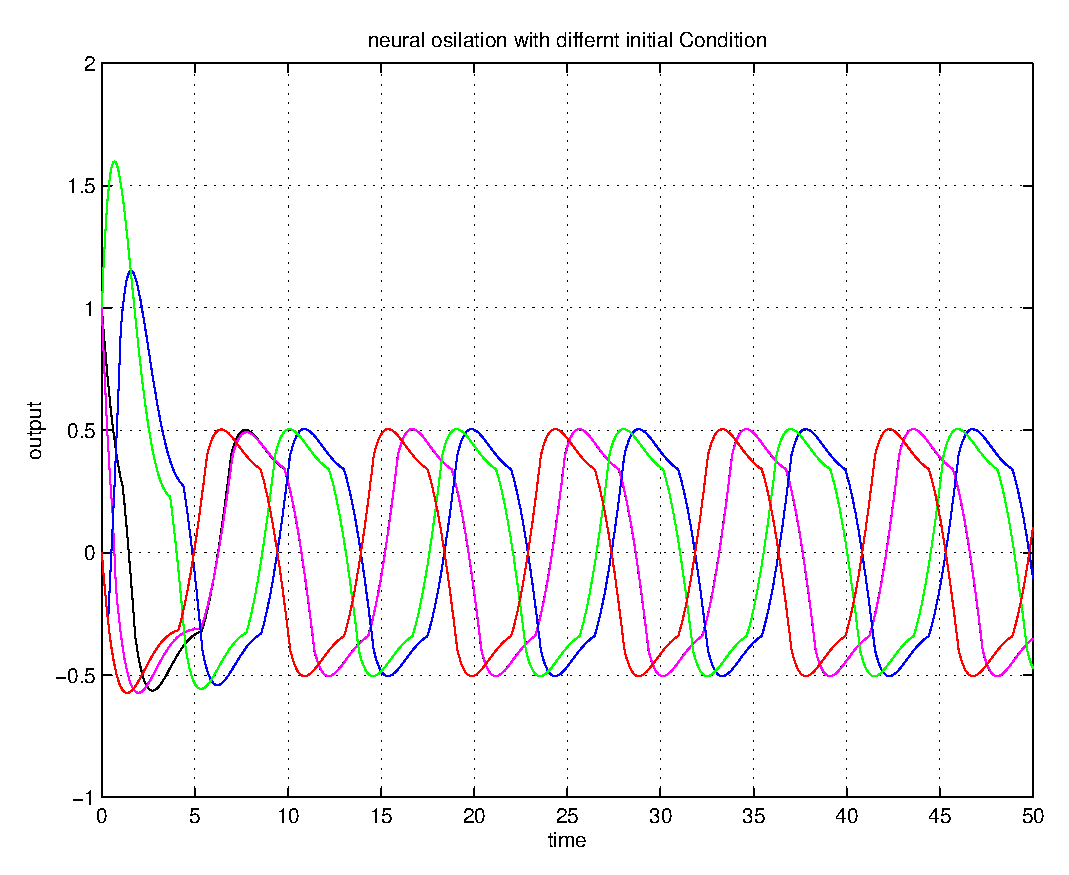
\includegraphics[width=1.5in]{\figurepath/neural_attraction.eps}
\label{fig:time_timeAttraction}
}
\hfill
\subfigure[Phase Portrait]{
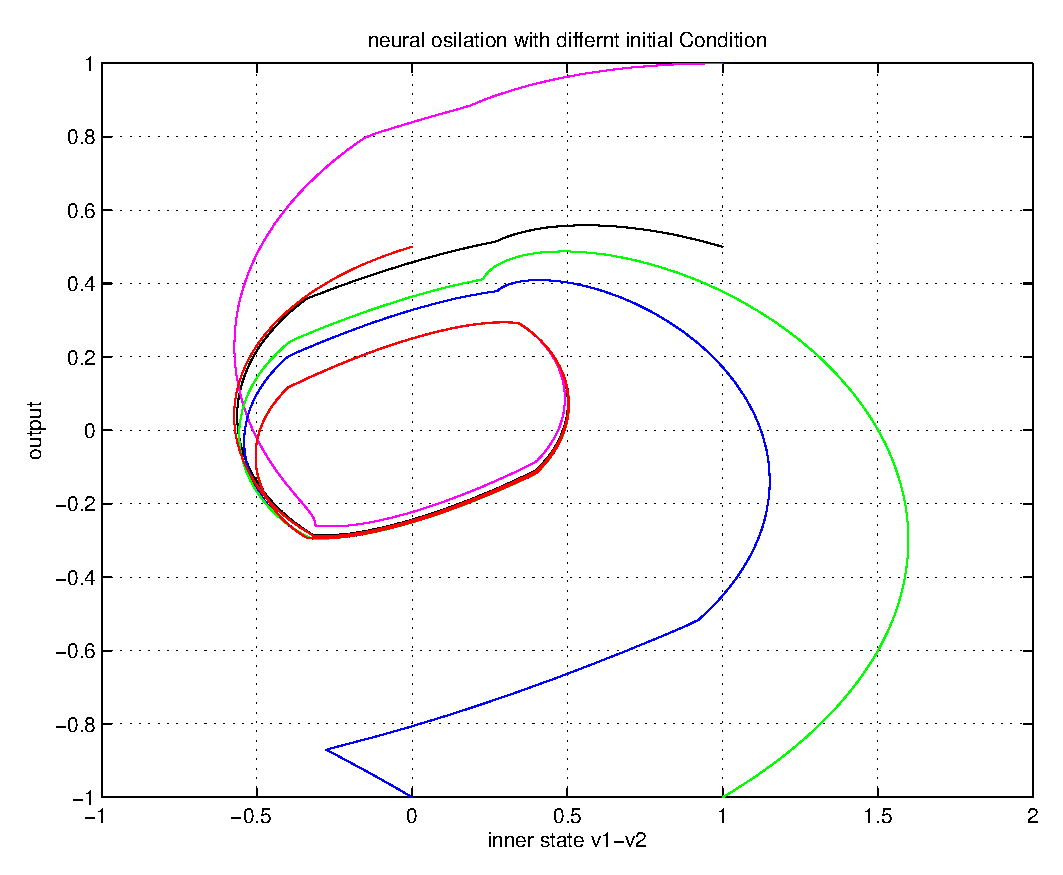
\includegraphics[width=1.5in]{\figurepath/neural_attraction_phase.eps}
\label{fig:phase_attraction}
}
}
\caption{Matsuta Oscilator}
\label{fig:matsuta oscilation}
\end{figure} 

Through this example, we believe neural oscillator is structure stable.
The large area of basin of attraction means the final behavior is totally determined by parameters. 
Initial conditions will have no effects on the final oscillation. 
The converging speed can be seen as quick recovery ability.
When an impulse perturbation happens, it will recover in one period time.

These properties are very valuable in CMS research. 
An intuitive idea is that we couple the neural oscillator with mechanical oscillator of body and environment, thus make the motion structual stable.

\section{Application to Bipedal Walking}
Bipedal walking is a common motion task and has been well studied by many research communities, including robotic \cite{Raibert1986}, artificial intelligence and biology as well as computer graphic research.
From experience, walking involves little reasoning activity, this idea is supported by the biology research that the number of neurons that take part in the lower limb control is very limited, much less than arm, hand and even tongue.
While for artificial system, robust bipedal walking is difficult to achieve. 
Many control method has been tried, but none of them shows comparable performance with human walking. 
In dynamic research,natural looking gaits can be generated by passive method.
There have been a series of passive dynamic walking machine\citep{McGeer1990,McGeer1990a}. 
If we put a passive walking machine on a slope, without any effort, it can walk down the slop. 
However the stabilities are very fragile. 
Passive walking can only be maintained when walking down a specific slope under specific condition.

From the viewport of Qualitative Control Theory, 
the reason why passive walking machines can walk down the slope is because that there exists a limit circle for the dynamic interaction between body and ground.
The fragile stability means the basin of attraction covers only a small area on the phase plane.
For natural looking walking motion,We plan to boost the stability of the passive walking machine by neural oscillation entrainment. 

\subsection{2D Passive Walking Model}
The mechanical model we adopted is illustrated in \figurename ~\ref{fig:2d_walker}. 
Both the model and simulation method are from the paper\citep{Wisse2005}. 
We only give brief description to make the content self-contained.

\begin{figure}
\begin{center}
\scalebox{0.5}{
\documentclass[11pt]{article}
\usepackage{pstricks,pst-eps}
\pagestyle{empty}
\begin{document}
\begin{TeXtoEPS}
\begin{pspicture}(0,-1)(10,10)
		%\psgrid
		
		\SpecialCoor
		\psline[linestyle=dashed](!0 -10 5 sin mul)(!10 5 cos mul  -10 5 sin mul)
		%\psgrid		
		\psline[linewidth=2pt]{->}(7,8)(7,6)
		\rput(6,7){$\mathbf g$}

		%\rput(2,7)
		%{
		% $\mathbf x_{n}$,$\mathbf y_{n}$ 	
		%}
		
		\rput{-5}(0,0)
		{
			%\psgrid
			%ground
			\psline[linewidth=3pt](0,0)(10,0)
			\psarc[linewidth=0.5pt]{<-}(10,0){9}{-180}{-175}
			%\psgrid
			\rput(0.5,-0.5){$\mathbf \gamma$}
			
						
			
			%\SpecialCoor
			%\psline[linewidth=0.5pt,linestyle=dashed](!2 10 cos 8 mul)(2,0)
			%\psline[linewidth=0.5pt](2,0.5)(1.5,0.5)
			%\psline[linewidth=0.5pt](1.5,0.5)(1.5,0)
						
			\SpecialCoor
			\rput{0}(!2 10 cos 8 mul)
			{	
				\psline[linewidth=3pt,linestyle=dashed](0,0)(0,6)
				%left leg		
				\rput{10}(0,0)
				{
					%\psgrid
					
					\psline[linecolor=blue,linewidth=3pt](0,0)(0,-4)
					\pscircle(0,0){0.1}
					\rput{0}(0,-4)
					{
					\psline[linecolor=blue,linewidth=3pt](0,0)(0,-4)
					\pscircle(0,0){0.1}
					\psdots[dotstyle=Bo,dotscale=3.0](0,-2)
					}
		
				
		
					
					\psline[linewidth=0.5pt](0,0)(-2.3,0)
					\psline[linewidth=0.5pt](0,-8)(-2.3,-8)
					\psline[linewidth=0.5pt]{<->}(-2,0)(-2,-8)
					\rput(-2.2,-4){ $\mathbf L$}
		
					\psline[linewidth=0.5pt](0,-2)(-1.1,-2)	
					\psline[linewidth=0.5pt]{<->}(-1,0)(-1,-2)
					\rput(-1.2,-1.5){$\mathbf b_{2}$}

					\psline[linewidth=0.5pt](0,-4)(-1.1,-4)	
					\psline[linewidth=0.5pt]{<->}(-1,-2)(-1,-4)
					\rput(-1.2,-3.5){$\mathbf a_{2}$}


					\psdots[dotstyle=Bo,dotscale=3.0](0,-2)
					\rput(0.7,-2.2){$\mathbf m_{s}$,$\mathbf I_{s}$}


					
					\rput{-5}(0,-8)
					{
					\psline[linewidth=0.5pt,linestyle=dashed](0.1,0)(0.1,4)
					\psarc[linewidth=0.5pt,linestyle=dashed]{->}(0.1,0){3.8}{90}{95}
					\rput(0.5,4.1){$\mathbf q_{1}$}
					}
					%\psarc[linecolor=blue,linewidth=3pt](0,-6){2}{210}{330}
					
				}
				%right leg
				\rput{40}(0,0)
				{
					%\psarc[linewidth=0.5pt,linestyle=dashed]{->}(0,0){5.5}{-150}{-90}
					%\SpecialCoor	
					%\rput(6;-105){$\mathbf \phi_{2}$}	
					\psline[linecolor=red,linewidth=3pt](0,0)(0,-4)
					\pscircle(0,0){0.1}
					\psdots[dotstyle=Bo,dotscale=3.0](0,-2)
					
					\rput{-35}(0,-4)
					{
					\psline[linewidth=0.5pt,linestyle=dashed](0,0)(0,1.5)
					\psarc[linewidth=0.5pt,linestyle=dashed]{->}(0,0){1}{90}{125}
					\rput(0.3,1){$\mathbf q_{2}$}
					}
					
					\rput{-10}(0,-4)
					{
					\psline[linecolor=red,linewidth=3pt](0,0)(0,-4)
					\pscircle(0,0){0.1}

				
					\psline[linewidth=0.5pt](0,0)(1.1,0)
					\psline[linewidth=0.5pt](0,-2)(1.1,-2)	
					\psline[linewidth=0.5pt]{<->}(1,0)(1,-2)
					\rput(1.2,-1.5){$\mathbf b_{1}$}

					\psline[linewidth=0.5pt](0,-4)(1.1,-4)	
					\psline[linewidth=0.5pt]{<->}(1,-2)(1,-4)
					\rput(1.2,-3.5){$\mathbf a_{1}$}
					\psdots[dotstyle=Bo,dotscale=3.0](0,-2)
					\rput(-0.7,-2){$\mathbf m_{t}$,$\mathbf I_{t}$}
					
					\rput{-25}(0,0)
					{
						\psline[linewidth=0.5pt,linestyle=dashed](0,0)(0,-1.5)
						\psarc[linewidth=0.5pt,linestyle=dashed]{->}(0,0){1.4}{270}{295}
						\rput(-0.3,-1){$\mathbf q_{3}$}
					}
					}

				}
				\psdots[dotstyle=Bo,dotscale=3.0](0,0)
				\rput(0.7,0){$\mathbf m_{H}$}
			}
		}
\end{pspicture}
\end{TeXtoEPS}


\end{document}



}
\caption{Passive Walking Model}
\label{fig:2d_walker}
\end{center}
\end{figure}

Passive walking is not a continuous dynamic system. 
We separate the motion into two phases and formulate two equations.

\textbf{Leg Swing Phase}
During the swing phases, we suppose that one leg is fixed on the ground, the arc foot makes the passive dynamic walker rolling without sliding.
The equation is 
\begin{equation}
\left[
\begin{array}{cc}
\bar{M} &D^{T}\\
D&	0 
\end{array}
\right]
\left[
\begin{array}{c}
\ddot{q} \\
F_{c}
\end{array}
\right]
=
\left[
\begin{array}{c}
\bar{F}\\
\ddot{D}\\
\end{array}
\right]
\end{equation}


\textbf{Heel Strike Phase}
We suppose the heel strike the ground in a short time, the angular momentum is preserved.
The Equation is as below
\begin{equation}
\left[
\begin{array}{cc}
\bar {M}& D^{T}\\
D	& 0
\end{array}
\right]
\left[
\begin{array}{c}
\dot{q}^{+}\\
f_{c}	
\end{array}
\right]
=
\left[
\begin{array}{c}
\bar{M}\dot{q}^{-}\\
0
\end{array}
\right]
\end{equation}
where $\dot{q}_{+}$ is the state variable after the collision, $\dot{q}_{-}$ is the state variable before the collision.



In the equations above,
\begin{eqnarray}
X=[x_{1},y_{1},\phi{1},x_{2},y_{2},\phi{2}]^{T} \nonumber\\
Q=[x_{h},y_{h},\phi{1},\phi{2}]^{T} \nonumber \\
T_{i,k}=\frac{\delta X_{i}}{ \delta Q_{k}} \nonumber \\
g(x)=\dot{T} \dot{q} \dot{q}	\nonumber \\
M=diag[m_{1} m_{1} I_{1} m_{2} m_{2} I_{2}] \nonumber \\
\bar{M}=T^{T}MT	\nonumber \\
\bar{f}=T^{T}[f-Mg]\nonumber \\
g_{y}=y_{h}-(l-r)*cos(\phi)-r=0 \nonumber \\
g_{x}=x_{h}+(l-r)*sin(\phi)+r*\phi-x_{f}\nonumber \\
D(x)=[g_{x}  g_{y}]^T=0 \nonumber
\end{eqnarray}

The input of neural oscillator is defined by the difference angle between the two legs.
\[
G_{input}=\phi_{1}-\phi_{2}
\]
Neural output will drive the biped walker. After adding the neural control, the equation of the dynamic system is
\begin{equation}
\left[
\begin{array}{cc}
\bar{M} &D^{T}\\
D&	0 
\end{array}
\right]
\left[
\begin{array}{c}
\ddot{q} \\
F_{c}
\end{array}
\right]
=
\left[
\begin{array}{c}
\bar{F}\\
\ddot{D}
\end{array}
\right]
+
\left[
\begin{array}{c}
\bar{U}\\
0	
\end{array}
\right]
\end{equation}

Neural oscillator output is applied at the hip joint to actuate the two legs towards different directions
\[
U=[0,0,1,-1]*G_{out}
\]

\subsection{Adaptive Walking Motion}

\textbf{Passive Walking}
When the passive walker walks down a slope, for every step, there is energy input from the potential energy,
and there is also energy loss because of heel strike. 
There must be an equilibrium condition when the energy lost is equal to the energy input. 
If natural looking motion is energy efficient, such passive walking motion can be expected to be natural looking. 
Because there is no extra control energy input, such motion is the most energy efficient.

\begin{figure}[H]
\centering
\includegraphics[width=3in]{\figurepath/passive_walking.eps}
\caption{Stable passive walking gait}
\label{fig:passive_walk}
\end{figure}
Figure \ref{fig:passive_walk} shows the gait of the passive walker. 
After coupling the neural oscillator, the basic pattern is not changed  as shown in \figurename ~\ref{fig:stable_active_walk}.

\begin{figure}[H]
\centering
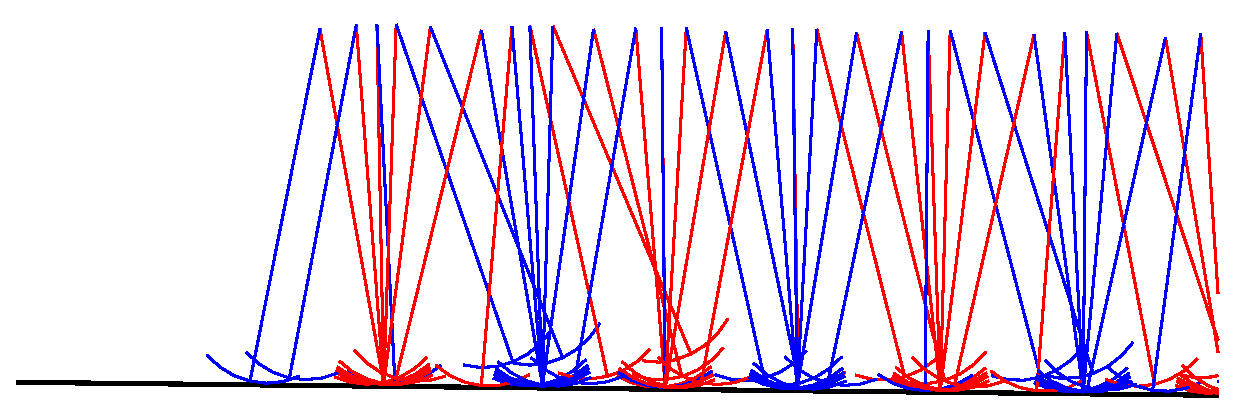
\includegraphics[width=3in]{\figurepath/actuated_walk_downslop.eps}
\caption{Walk down the same slop when actuated}
\label{fig:stable_active_walk}
\end{figure}

\textbf{Walking On Plain}
However the stability is fragile.  
The passive walker can't walk on plane. 
The step size will decrease after each step, and finally it will stop or fall over as illustrated in \figurename ~\ref{fig:pass_waling_on_plane}.
\begin{figure}[!h]
\centering
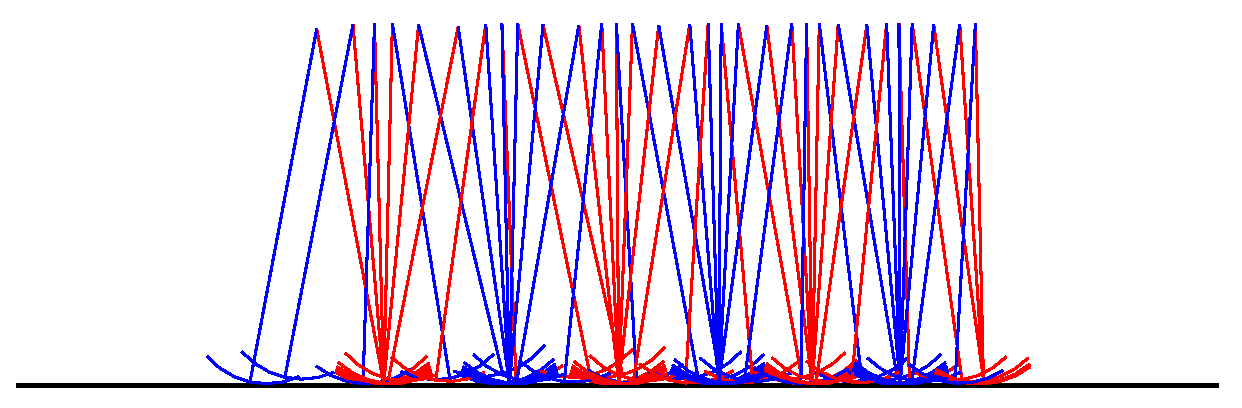
\includegraphics[width=3in]{\figurepath/passive_walk_on_plane.eps}
\caption{Passive walking gait can't be maintained on plane}
\label{fig:pass_waling_on_plane}
\end{figure}

After coupled with the neural oscillator, this walking machine can walk on plane, and exhibits gait similar to the passive dynamic walker. 
\figurename ~\ref{fig:walk_plane} shows the gait. 
From the state plot \figurename ~\ref{fig:walk_plane_state}, and phase plot \figurename ~\ref{fig:walk_plane_phase}, we can see that the gait converged to a stable limit circle.


\begin{figure}[!h]
\centering
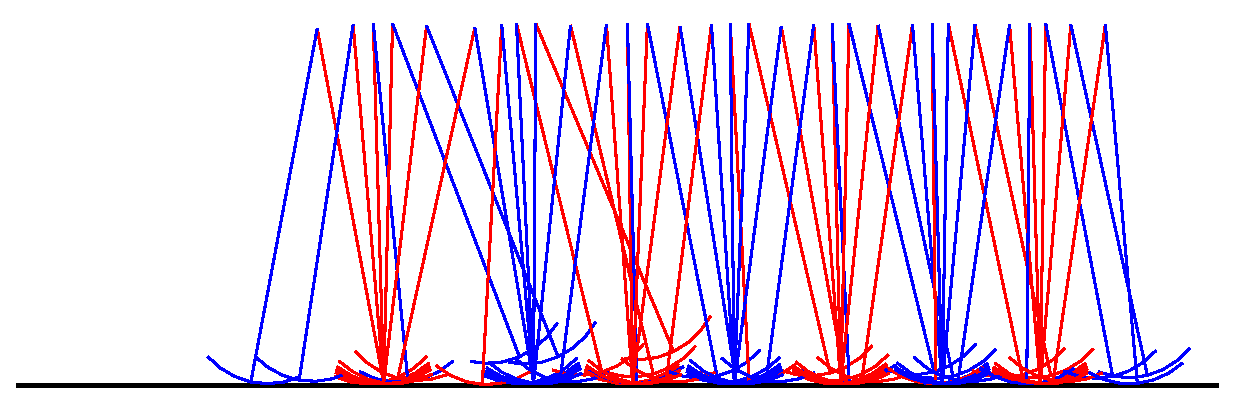
\includegraphics[width=3in]{\figurepath/walker_on_plane.eps}
\caption{Walking on plane under neural control}
\label{fig:walk_plane}
\end{figure}


\begin{figure}[!h]
\centerline{
\subfigure[State Plot]{
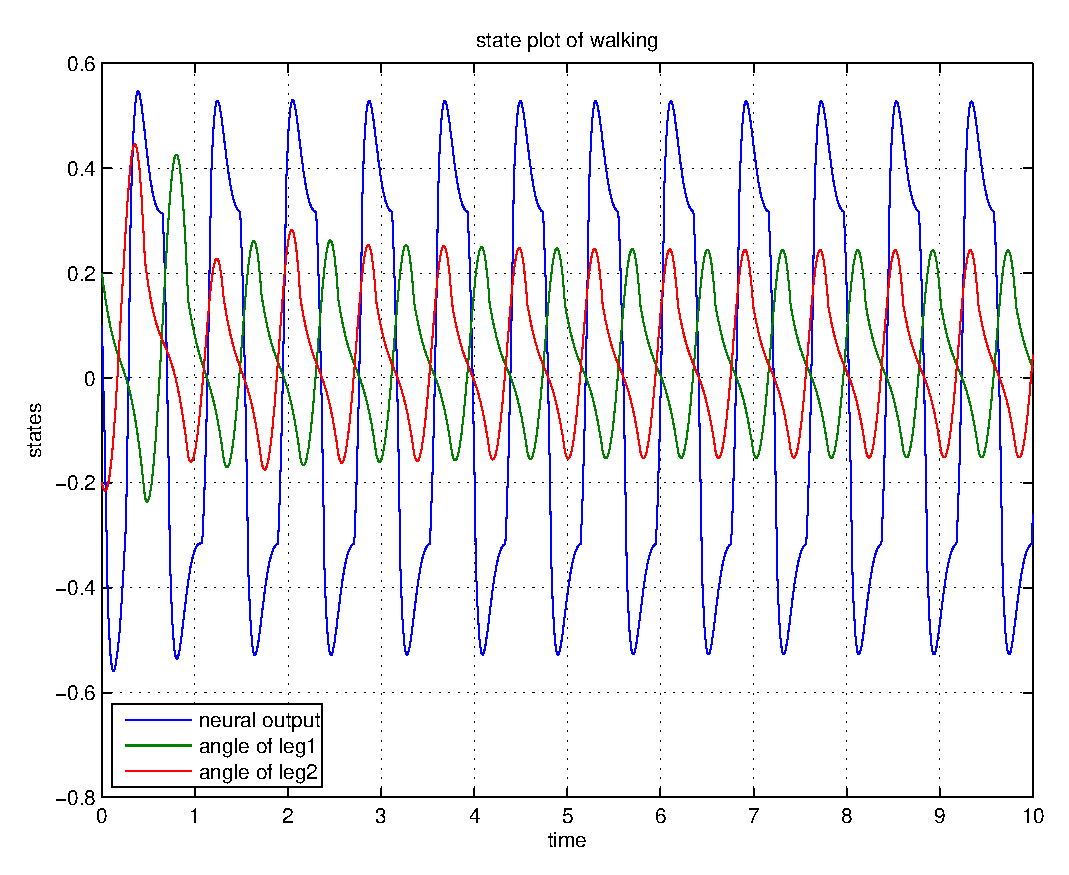
\includegraphics[width=1.5in]{\figurepath/walking_on_plane_time_state}
\label{fig:walk_plane_state}
}
\hfill
\subfigure[Phase Plot]{
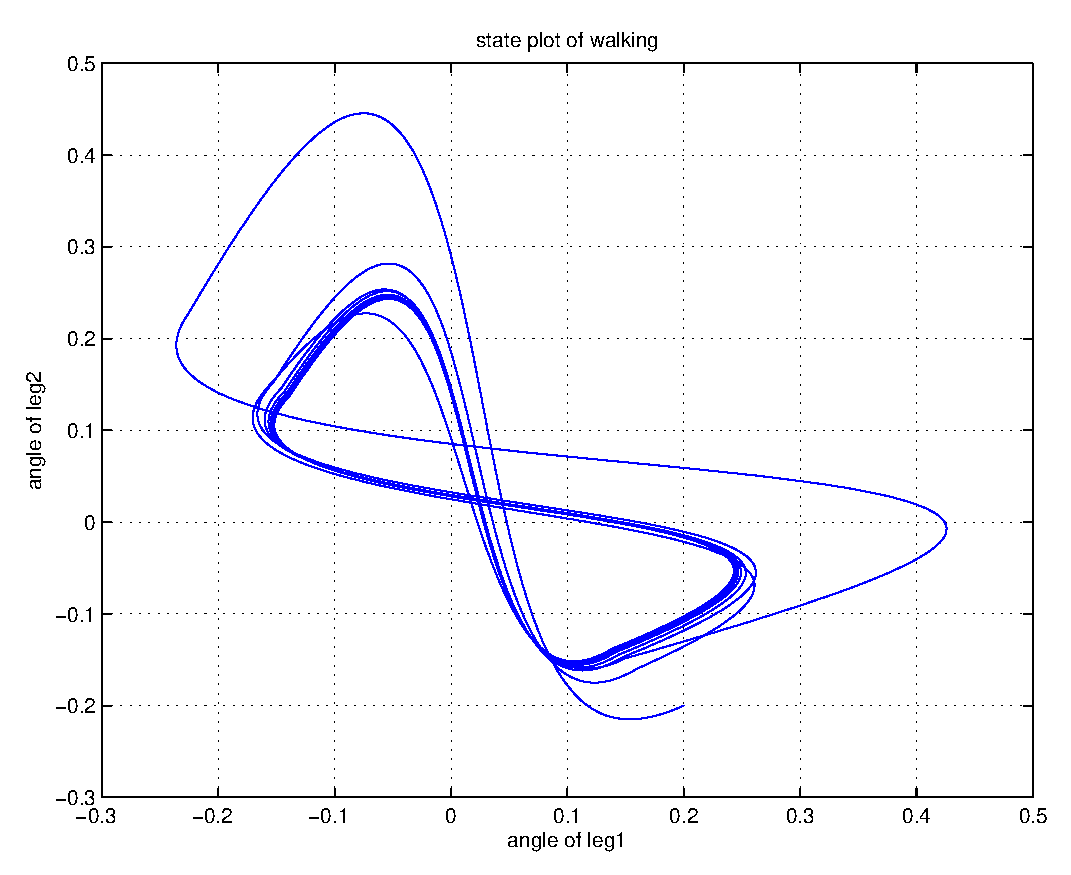
\includegraphics[width=1.5in]{\figurepath/walking_on_plane_phase.eps}
\label{fig:walk_plane_phase}
}
}
\caption{
Walking on a plane converges to a stable limited circle
}
\label{fig:walk_on_plane}
\end{figure}

To verify the structural stability, we introduce a variety of perturbations to the passive walker. 
These perturbations include different initial condition, different slopes, different leg mass and different leg length.

\textbf{Different Initial Condition}
The original passive walker is not very stable. 
A slight change in initial condition will result in walking failure. 
While after coupled with neural oscillator, the basin of attraction has been enlarged. 
A different initial condition can still lead to a stable gait, as show in Figure \ref{fig:diff_init}. 
Natural looking gait is maintained.
\begin{figure}[h]
\centering
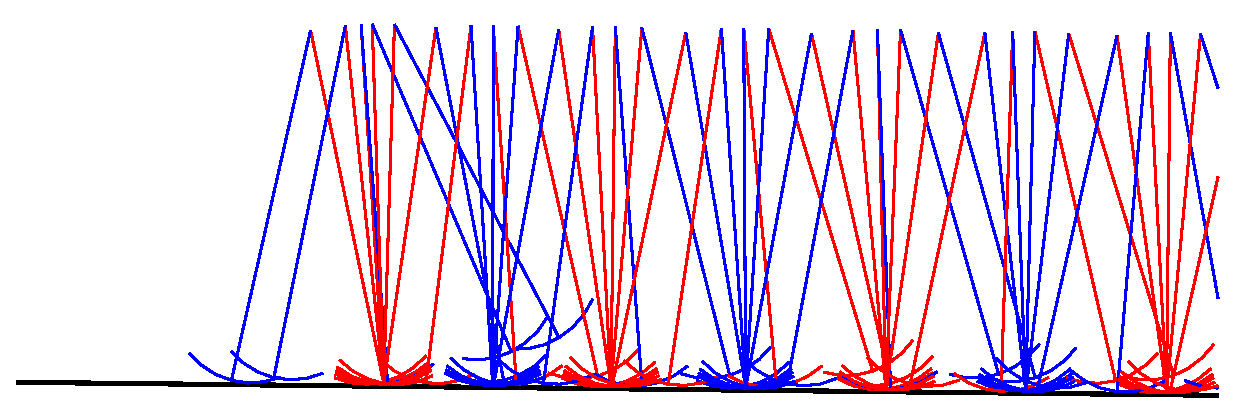
\includegraphics[width=3in]{\figurepath/walk_down_with_differnt_init_cond_suceed.eps}
\caption
{
Walking with different Initial condition
}
\label{fig:diff_init}
\end{figure}
 

\textbf{Walking On Different Slopes}
Another parameter we change is angle of the walking slope. 
When we increase the down slope, stable walking motion can still be maintained, as shown in figure \ref{fig:diff_slop}.
An important discovery is that although the walkers can walk on various down slopes, it can not walk up slope,no matter how control parameters are changed.
It can’t walk up slope and will fall backward after several steps. 
We suggest that this is because the proper limit circle does not exist in the dynamic system when walking up slope.
This finding may help us to understand the upper body effect in walking.

\begin{figure}[h]
\centering
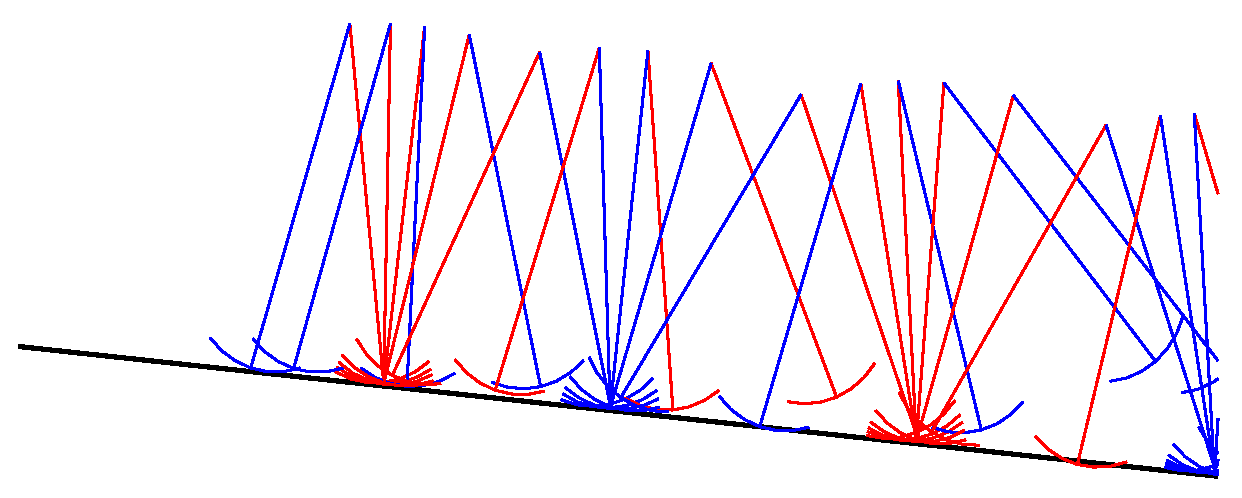
\includegraphics[width=3in]{\figurepath/big_slop_actuated_suceed.eps}
\caption
{
Walking with different slope angle
}
\label{fig:diff_slop}
\end{figure}

\textbf{Leg Mass Variation}
We add mass on one leg to 50\% and find the stability of the gait is still maintained. 
The step length and swing period of the two legs are different, this gait is similar to that with a crippled leg, see figure\ref{fig:leg mass}.

\begin{figure}[H]
\centering
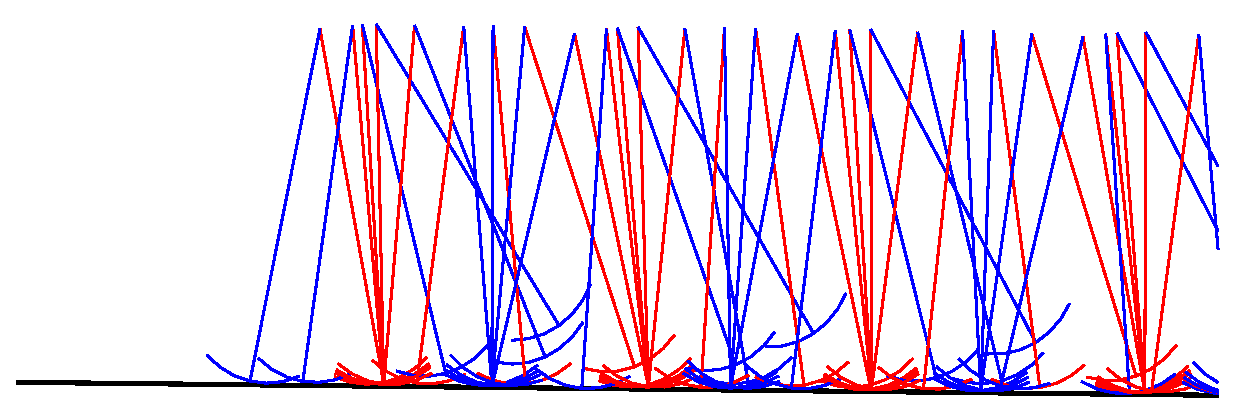
\includegraphics[width=3in]{\figurepath/walk_mass_changed.eps}
\label{fig:walk_mass_changed}
\caption
{
Walking with legs of different mass
}
\label{fig:leg mass}
\end{figure}

\textbf{Leg Length Variation}
The last parameter we change is the leg length. 
We change the leg length to 1/8 shorter. 
And we find the stability of the gait is maintained, see \figurename ~\ref{fig:walk_leg_changed}

\begin{figure}[H]
\centering
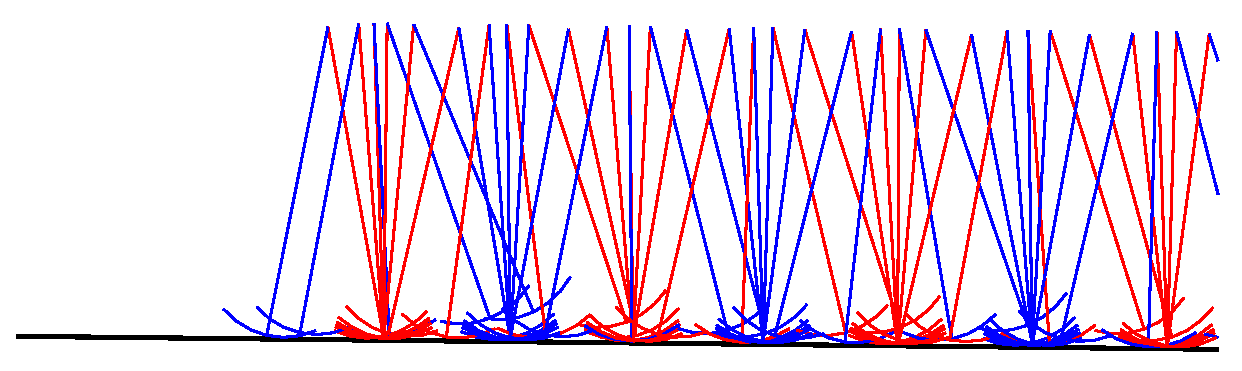
\includegraphics[width=3in]{\figurepath/walk_leg_changed_success.eps}
\caption
{
Walking with shorter Legs
}
\label{fig:walk_leg_changed}
\end{figure}






\section{Discussion and Future Work}
Qualitative Control Theory can synthesize motion with adaptive behaviour while keeping the qualitative properties of motion.
It provides a new method to synthesize adaptive motion efficiently. Since very little computation involved in each controller, compared with traditional optimiaztion based method, this method can generate motions in realtime. And most importantly, our method is parallel in nature. Each CPG only control on single degree of freedom. For complicate characters, many different CPGs can be simulated in parallel without referencing each other. Since many physical simulation modules have been implemented efficiently using GPU, in future, most of the computational burden of our method can be shifted to GPU. This will make our algorithm generating agile motions even with very complicated environment and involving whole body structures. 


However since we bring in a new theory into the motion synthesis area, many works need to be done in the future. For example, our current model only involves the lower body structure, upper body and more joints will be considered in our future design. To proof the adaptivness, we will need experiment on more complicate terrian instead of just upslope and downslope.

More Central Pattern Generators are needed for different kinds of motions. And how to turn the CPG parameters for the animator purpose are still open.
These topics will be covered in the future research.







\bibliographystyle{plainnat}
\bibliography{rommePaper}




\end{document}


